\section{Results}
\label{sec:results}

% Subsections still to be written by their owners:
%   - SAE reconstruction and sparsity
%   - Layer-wise probe performance
%   - Causal intervention outcomes

\subsection{Free-form feedback made the Solver adopt almost everything}
\label{sec:res-protocol}

Under the free-form protocol, the Solver almost always followed the Critic
(Table~\ref{tab:protocol}). Retention was too rare to train a probe on: 8\%
of the binary cohort under the rule-based labels and 3\% under the
LLM-derived labels. The candidate presentation, with the same questions and
models, brought the Adoption share down to 54.8\%, which gives a usable
binary target. This is why every later collection uses the candidate
presentation.

\begin{table}[htbp]
    \centering
    \caption{Adoption share of the binary cohort under the two Solver
    protocols. The free-form rows use the training partition (rule-based) or
    a 1,000-episode sample (LLM-derived); the candidate row uses the full
    collection.}
    \label{tab:protocol}
    \begin{tabular}{llrr}
        \toprule
        Protocol & Label source & Binary episodes & Adoption share \\
        \midrule
        Free-form feedback & Rule-based (earlier rules) & 4,177 & 91.7\% \\
        Free-form feedback & LLM-derived                &   586 & 97.3\% \\
        Candidate presentation & Rule-based (final rules) & 10,644 & 54.8\% \\
        \bottomrule
    \end{tabular}
\end{table}

\subsection{Candidate order shifts the Adoption--Retention balance}
\label{sec:res-order}

Presentation order changes the Solver's choice. When the Critic's
recommendation is listed first, the Adoption share of the binary cohort is
57.8\% (95\% CI 56.4--59.1), against 51.9\% (50.5--53.2) when A1 is listed
first (Table~\ref{tab:order}). The gap appears in every partition, with the
Critic-first share higher by 4 to 9 percentage points
(Figure~\ref{fig:order}).

\begin{figure}[htbp]
    \centering
    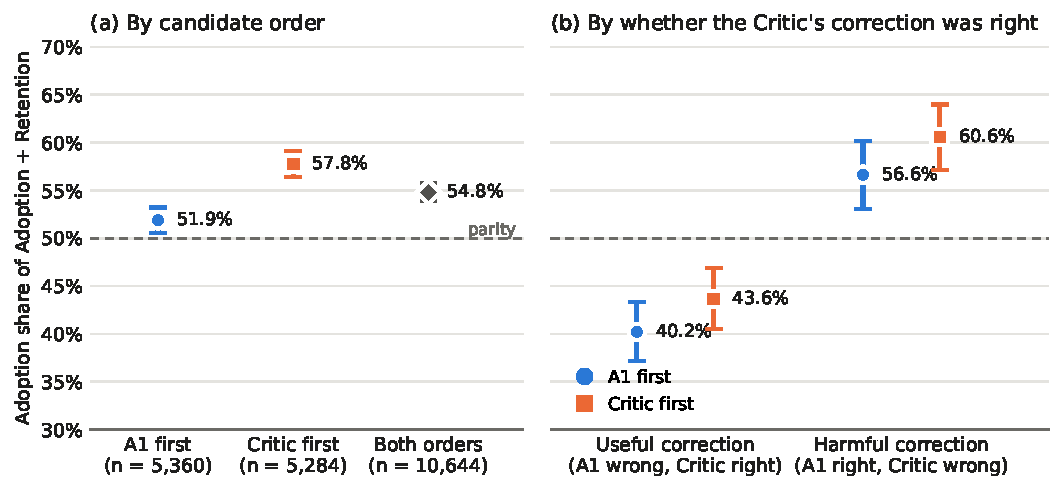
\includegraphics[width=0.85\linewidth]{../../reports/figures/candidate_order_balance/candidate_order_adoption.pdf}
    \caption{Adoption share of the binary cohort by candidate order, with 95\%
    Wilson intervals (rule-based reference labels).}
    \label{fig:order}
\end{figure}

\begin{table}[htbp]
    \centering
    \caption{Adoption share of the binary cohort (Adoption / (Adoption +
    Retention)) by candidate order, rule-based reference labels, with 95\%
    Wilson intervals.}
    \label{tab:order}
    \begin{tabular}{lcc}
        \toprule
        Partition & A1 first & Critic first \\
        \midrule
        Train        & 51.5\% (50.0--53.1) & 57.4\% (55.9--59.0) \\
        Validation   & 53.5\% (49.3--57.5) & 58.6\% (54.5--62.7) \\
        Test         & 51.5\% (47.0--56.1) & 60.2\% (55.8--64.4) \\
        Intervention & 53.1\% (48.7--57.4) & 57.0\% (52.5--61.4) \\
        \midrule
        All          & 51.9\% (50.5--53.2) & 57.8\% (56.4--59.1) \\
        \bottomrule
    \end{tabular}
\end{table}

Because orders are assigned in equal numbers, the effect largely cancels in
the overall label mix. It still matters for the probes. A probe could
predict Adoption partly from which candidate came first, so candidate order
should be reported as a baseline feature and checked as a confound in every
probe and feature analysis.

\subsection{Synthetic questions produce little disagreement}
\label{sec:res-synthetic}

The synthetic questions did not behave like MuSiQue questions
(Figure~\ref{fig:synthetic}, Table~\ref{tab:synthetic-pilot}). Only 16 of 100 synthetic episodes were
Adoption or Retention, against 56 of 100 matched MuSiQue episodes, and the
two 95\% intervals do not overlap. The difference arises before the Solver
ever sees the feedback. The Solver answered 78\% of synthetic questions
correctly on its first attempt, and the Critic 90\%, so in most episodes
both agreed on the right answer.

\begin{figure}[htbp]
    \centering
    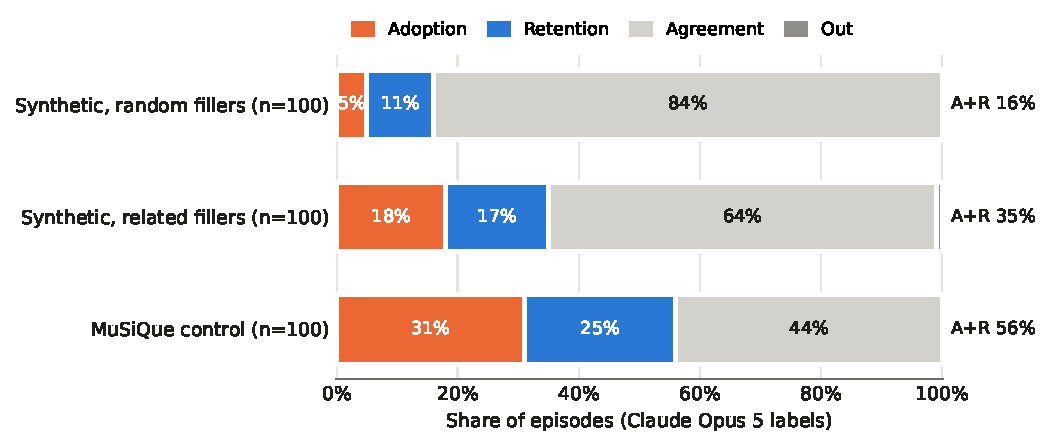
\includegraphics[width=\linewidth]{../../reports/figures/synthetic_pilot/synthetic_vs_musique_behavior.pdf}
    \caption{Behavior labels for the synthetic pilot with its original (random)
    fillers, the same questions with related fillers, and a hop-matched MuSiQue
    control (LLM-derived labels, $n = 100$ each).}
    \label{fig:synthetic}
\end{figure}

\begin{table}[htbp]
    \centering
    \caption{Synthetic pilot, paired filler ablation, and hop-matched MuSiQue
    control (LLM-derived labels, $n = 100$ each). One related-filler question
    was excluded at collection because the Critic gave no recommendation; it is
    counted as Out, and accuracies use the 99 collected episodes.}
    \label{tab:synthetic-pilot}
    \begin{tabular}{lrrr}
        \toprule
         & \multicolumn{2}{c}{Synthetic} & MuSiQue \\
        \cmidrule(lr){2-3}
         & Random fillers & Related fillers & \\
        \midrule
        Adoption  &  5 & 18 & 31 \\
        Retention & 11 & 17 & 25 \\
        Agreement & 84 & 64 & 44 \\
        Out       &  0 &  1 &  0 \\
        \midrule
        Adoption + Retention (95\% CI) & 16\% (10--24) & 35\% (26--45) & 56\% (46--65) \\
        Adoption share of the binary cohort & 31\% & 51\% & 55\% \\
        A1 correct & 78\% & 65\% & 21\% \\
        Critic correct & 90\% & 89\% & 27\% \\
        \bottomrule
    \end{tabular}
\end{table}

A follow-up analysis of the same episodes points to several causes, none
dominant on its own:
\begin{itemize}
    \item \textbf{Weak fillers.} The filler paragraphs rarely compete with
    the evidence. A synthetic question has 1.5 non-supporting paragraphs on
    average that share two or more of its content words, against 10.7 for
    MuSiQue. A lexical retriever ranks every supporting paragraph near the
    top (within the first hops + 2 positions) for 74\% of synthetic questions,
    against 16\% for MuSiQue.
    \item \textbf{Scoring.} Strict string matching undercounts MuSiQue
    accuracy, because many MuSiQue first answers are full sentences. With
    lenient matching, A1 accuracy is 83\% for synthetic and 35\% for
    MuSiQue, so about 10 of the 57-point gap is a scoring artifact.
    \item \textbf{Defects in MuSiQue.} Part of MuSiQue's disagreement comes
    from defects in the dataset itself: garbled composed questions, gold
    answers that do not fit the question, and paragraphs that do not state
    the cited relation. The Critic refused to answer 17\% of the control
    questions and none of the synthetic ones.
\end{itemize}

MuSiQue's Adoption + Retention rate is therefore not the right target for
the synthetic data. Most synthetic disagreements are the clean case, a
wrong A1 that the Critic corrects (12 of 16), whereas more than half of
MuSiQue's disagreements involve two wrong answers (32 of 56). The goal is
enough clean disagreement, not a match to MuSiQue's rate.

\subsection{Related fillers}
\label{sec:res-fillers}

Replacing only the filler paragraphs more than doubled the useful
disagreement: Adoption + Retention rose from 16\% to 35\% of episodes
(Table~\ref{tab:synthetic-pilot}). Pairing the same questions across the two
conditions, 22 episodes became Adoption or Retention and 3 stopped being so
(exact McNemar test, $p < 0.001$). The Adoption share of the binary cohort
also moved from 31\% to 51\%, close to MuSiQue's 55\%.

The related fillers act mainly on the Solver's first answer. A1 accuracy fell
from 78\% to 65\%, while the Critic stayed near 90\%. In 17 of the 22 new
disagreements the Solver was wrong and the Critic right, which is the clean
case of correctable feedback. The new wrong answers are genuine reasoning
errors rather than noise: of 19, twelve take an intermediate entity or the
wrong span from a supporting paragraph, four take an answer from a related
filler, two from a generated distractor, and one appears nowhere in the
context.

Two checks support attributing the change to the fillers. Collecting the
original questions again in the same environment reproduced every A1, Critic
answer, and A2 of the original pilot exactly. On the 57 episodes whose three
answers did not change, the labeler assigned the same label in every case.
